\section{Method: Width-Thresholded Geometry and Asynchronous Execution}
\label{sec:method}

Directly translating the two structural laws from \Cref{sec:diagnosis} into an optimizer and distributed runtime yields \mname{WT-MLP-Lag}.
We first specify the unified two-sided operator family and width-thresholded factorization (\Cref{sec:operator}), then detail the three-pillar systems co-design that hides critical-path cotangent latency across $8\text{--}32\times\text{A100}$ (\Cref{sec:systems}).

\subsection{Unified Two-Sided Operator Family and Width Thresholding}
\label{sec:operator}

For each 2D Transformer block projection $p \in \{\text{q, k, v, o, gate, up, down}\}$ of shape $m_p \times n_p$ with globally averaged gradient $G_{p,t} \in \R^{m_p \times n_p}$, we maintain standard Nesterov momentum without $(1-\mu)$ dampening:
\begin{equation}
  M_{p,t} = \mu M_{p,t-1} + G_{p,t}, \qquad U_{p,t} = G_{p,t} + \mu M_{p,t}, \qquad \mu = 0.95,\quad M_{p,-1} = 0.
  \label{eq:momentum}
\end{equation}
Let $\Nten:\R^{m \times n} \to \R^{m \times n}$ denote the executed 10-step quintic Newton--Schulz map with coefficients $(3.4445,\,-4.7750,\,2.0315)$, Frobenius normalization floor $10^{-5}$, and BF16-operand / FP32-accumulate GEMMs (\texttt{tpu} mode; exact specification in \Cref{app:appendix_math}).
Given right (input) inner/outer factors $(R_{p,t},\,\hat{R}_{p,t}) \in \R^{n_p \times n_p}$ built from $C_{g(p),t}$ and left (output) inner/outer factors $(L_{p,t-\tau},\,\hat{L}_{p,t-\tau}) \in \R^{m_p \times m_p}$ built from $B_{p,t-\tau}$ at lag $\tau \in \{0, 1\}$, every method in our study updates $W_{p,t}$ via
\begin{equation}
  D_{p,t} = \hat{L}_{p,t-\tau}\,\Nten\!\left(L_{p,t-\tau}\,U_{p,t}\,R_{p,t}\right)\hat{R}_{p,t},
  \qquad
  W_{p,t+1} = W_{p,t} - \eta_t\left(s_{m_p,n_p}\,D_{p,t} + \lambda\,Q_{p,t}\right),
  \label{eq:update}
\end{equation}
where $s_{m,n} = \sqrt{\max(1, m/n)}$ ($s=2$ for tall \texttt{gate, up}; $s=1$ otherwise), $\lambda = 0.1$ is the decoupled weight-decay coefficient, and $Q_{p,t} = W_{p,t}\hat{R}_{p,t}^2$ when right outer factors are active (falling back to $\hat{L}_{p,t-\tau}^2 W_{p,t}$ for left-only ablations and $W_{p,t}$ for \mname{Muon}).
Embeddings, the untied output head, and RMSNorm gains remain routed to auxiliary AdamW cleanly separated from \Cref{eq:update}.

\paragraph{Dense vs.\ diagonal factor operators and scale preservation.}
Each active factor slot in \Cref{eq:update} instantiates \Cref{eq:trace_norm} in either dense spectral form ($\mathsf{Dense}$) or elementwise diagonal form ($\mathsf{Diag}$, using $f = \diag(F)$ and $a = d\,f/(\mathbf{1}^{\Tr}f) + \epsilon\mathbf{1}$):
\begin{align}
  L^{\mathsf{Dense}} &= A_m(B)^{-1/2}, &
  \hat{L}^{\mathsf{Dense}} &= \unitrms\!\bigl(A_m(B)^{-1/8}\bigr), \label{eq:dense_roots}\\
  L^{\mathsf{Diag}} &= \Diag\!\bigl(a(B)^{-1/2}\bigr), &
  \hat{L}^{\mathsf{Diag}} &= \unitrms\!\bigl(\Diag(a(B)^{-1/8})\bigr), \label{eq:diag_roots}
\end{align}
where $\unitrms(X) \triangleq \sqrt{d}\,X / \|X\|_F$ enforces $\frac{1}{d}\|\unitrms(X)\|_F^2 = 1$ (with zero-trace startup moments returning $I_d$).
Two deliberate design choices distinguish \Cref{eq:update,eq:dense_roots,eq:diag_roots} from prior two-sided proposals:
\begin{enumerate}[leftmargin=1.6em, itemsep=2pt, topsep=2pt]
  \item \textbf{Decoupled $(-1/2,\,-1/8)$ powers with unit-RMS outer scaling (no global norm grafting).}
  Matching \mname{MuonT}'s input recipe, the unnormalized $-1/2$ inner factor whitens the singular frame \emph{entering} $\Nten$ (where $\Nten$'s initial Frobenius normalization absorbs global scale), while the gentler unit-RMS $-1/8$ outer factor reweights output coordinates \emph{after} $\Nten$ without inflating the update Frobenius norm ($\|D\|_F / \|D_{\text{MuonT}}\|_F = 0.985$; \Cref{sec:mechanism}).
  Consequently, \mname{MuonT}'s learning rate transfers directly without ad-hoc post-hoc Frobenius norm grafting.
  \item \textbf{Retaining input-shaped weight decay $Q_{p,t} = W_{p,t}\hat{R}_{p,t}^2$.}
  Modifying $Q_{p,t}$ simultaneously with $D_{p,t}$ confounds descent geometry with regularization strength. Keeping $Q_{p,t}$ identical to \mname{MuonT} isolates the pure effect of output-preconditioned descent directions (we separately ablate isotropic decay in \Cref{sec:related_baselines}).
\end{enumerate}

\begin{table}[t]
  \centering
  \caption{\textbf{Taxonomic specification of the core optimizer methods and matched falsification controls} under the unified update rule \Cref{eq:update}. Widths $(\dm, \dff)$ equal $(512, 2048)$ at \texttt{130M} and $(1024, 4096)$ at \texttt{520M}. Additional structural ablations (\mname{Abl-*}) are defined and evaluated in \Cref{sec:ablations}.}
  \label{tab:taxonomy}
  \vspace{2pt}
  \resizebox{\textwidth}{!}{%
  \begin{tabular}{@{}llccccc@{}}
    \toprule
    \multirow{2}{*}{Method} & \multirow{2}{*}{Role in Study} & \multicolumn{2}{c}{Right Input Factors $R, \hat{R}$} & \multicolumn{2}{c}{Left Output Factors $L, \hat{L}$} & \multirow{2}{*}{Lag $\tau$} \\
    \cmidrule(lr){3-4} \cmidrule(lr){5-6}
    & & $\dm$ (\texttt{attn,o,mlp}) & $\dff$ (\texttt{down}) & $\dm$ (\texttt{q,k,v,o,down}) & $\dff$ (\texttt{gate,up}) & \\
    \midrule
    \mname{Muon}        & Orthogonalized baseline    & $I$     & $I$     & $I$     & $I$     & --- \\
    \mname{MuonT}       & Input-whitened baseline    & Dense   & Dense   & $I$     & $I$     & --- \\
    \midrule
    \mname{OD-All}      & Pure-diagonal output limit & Dense   & Dense   & Diag    & Diag    & $0$ \\
    \mname{WT-Sym-Lag}  & Symmetric $\dff$ threshold & Dense   & Diag    & Dense   & Diag    & $1$ \\
    \rowcolor{rowtint}
    \textcolor{colWT}{\mname{WT-MLP}}     & \textcolor{colWT}{\textbf{Width-thresholded (sync)}} & \textcolor{colWT}{\textbf{Dense}} & \textcolor{colWT}{\textbf{Dense}} & \textcolor{colWT}{\textbf{Dense}} & \textcolor{colWT}{\textbf{Diag}} & \textcolor{colWT}{\textbf{$0$}} \\
    \rowcolor{rowtint}
    \textcolor{colWT}{\mname{WT-MLP-Lag}} & \textcolor{colWT}{\textbf{Proposed primary method}}  & \textcolor{colWT}{\textbf{Dense}} & \textcolor{colWT}{\textbf{Dense}} & \textcolor{colWT}{\textbf{Dense}} & \textcolor{colWT}{\textbf{Diag}} & \textcolor{colWT}{\textbf{$1$}} \\
    \mname{DT-All} / \mname{-Lag} & Dense two-sided ceiling & Dense & Dense & Dense   & Dense   & $0 / 1$ \\
    \midrule
    \mname{Null-WT}     & Matched-path control for \mname{WT} & Dense & Dense & \multicolumn{2}{c}{Captured \& rooted, $I$ applied} & $0$ \\
    \mname{Null-Dense}  & Matched-path control for \mname{DT} & Dense & Dense & \multicolumn{2}{c}{Captured \& rooted, $I$ applied} & $0$ \\
    \bottomrule
  \end{tabular}%
  }
\end{table}

\paragraph{Width-thresholded output assignment (\mname{WT-MLP} and \mname{WT-MLP-Lag}).}
\Cref{tab:taxonomy} summarizes how our primary method and key comparison arms populate \Cref{eq:update} (\Cref{fig:method_pipeline}a):
\mname{WT-MLP} retains \mname{MuonT}'s full dense input factors across all four input groups, assigns dense spectral roots \eqref{eq:dense_roots} to all five hidden-width ($\dm$) outputs (\texttt{q, k, v, o, down}), and assigns exact elementwise diagonal roots \eqref{eq:diag_roots} to the two expanded ($\dff$) pre-SwiGLU outputs (\texttt{gate, up}).
This single architectural threshold eliminates both $\dff \times \dff$ output eigendecompositions per layer ($96.2\%$ of output $O(d^3)$ work and $0.50\text{ GiB}$ of packed Grams), while recomputing \texttt{gate} and \texttt{up} coordinate scales \emph{exactly} every step without cached-basis staleness.

\begin{figure}[t]
  \centering
  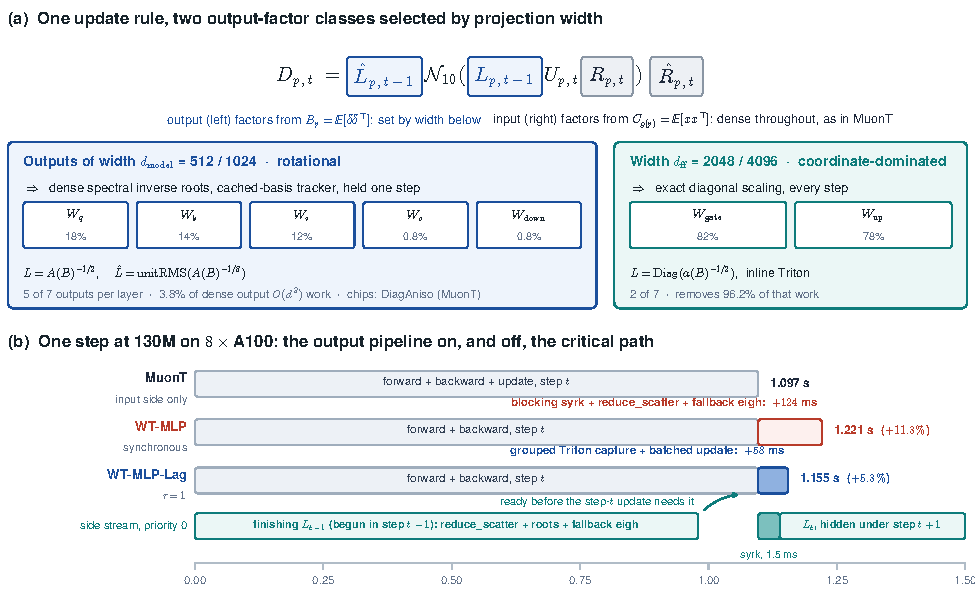
\includegraphics[width=\textwidth]{fig3_method_pipeline.pdf}
  \caption{\textbf{Factor assignment and execution pipeline of \mname{WT-MLP-Lag}.}
  \textbf{(a)} The four factor slots of \Cref{eq:update}. Right input factors stay dense for every projection, as in \mname{MuonT} (grey); the left output factor is chosen by the width of the cotangent, dense spectral roots at $\dm$ (blue) and exact per-step diagonal scaling at $\dff$ (teal). Chip labels give each moment's $\mathrm{DiagAniso}$ on the \mname{MuonT} trajectory (\Cref{tab:diagnosis}), the measurement that sets the threshold.
  \textbf{(b)} One training step at \texttt{130M} on $8\times\text{A100}$, drawn to scale from the median step times of \Cref{tab:bench19}. Synchronous two-sided execution appends \texttt{syrk}, \texttt{reduce\_scatter}, and fallback \texttt{eigh} to the step boundary, since $\delta_t$ exists only after backward completes. At $\tau=1$ the step-$t$ update instead consumes $L_{t-1}$, and the output pipeline runs on a priority-0 side stream: \texttt{syrk} ($\sim 1.5\text{ ms}$, guarded by \texttt{ev\_rows\_consumed}) followed by reduction and root updates for $L_t$ hidden under step $t+1$. Only the step bars are to scale; side-stream extents are schematic.}
  \label{fig:method_pipeline}
\end{figure}

\subsection{Systems Co-Design: Hiding Critical-Path Cotangent Latency}
\label{sec:systems}

Even after width thresholding removes $\dff$-wide eigendecompositions, executing five $\dm$-wide dense output roots synchronously (\mname{WT-MLP}) still adds $+11.3\%$ benchmark step-time overhead ($+21.9\%$ in early unbatched runs) because cotangents $\delta_t$ exist only \emph{after} backward completes (\Cref{fig:method_pipeline}b, middle row).
Our production engine (\texttt{fast\_lag}) eliminates this bottleneck via three orthogonal systems optimizations:

\paragraph{1. One-step asynchronous lag ($\tau = 1$), non-blocking masked repairs, and batched fallback \texttt{eigh}.}
In \mname{WT-MLP-Lag}, step $t$ applies step $t-1$'s already-computed output roots $(L_{p,t-1}, \hat{L}_{p,t-1})$ while keeping input roots $(R_{p,t}, \hat{R}_{p,t})$ current ($t=0$ uses identity left factors for $1$ step out of $5{,}120$).
At $\beta = 0.938$, a 1-step delay shifts the exponential weighting window by a single update out of $\approx 16.1$, costing $< 10^{-3}$ nats in held-out loss (\Cref{sec:ablations}).
Systems-wise, however, $\tau = 1$ moves the entire output pipeline off the critical path (\Cref{fig:method_pipeline}b, bottom two rows):
once backward $t$ finishes, a normal-priority ($\text{priority}=0$) CUDA side stream---chosen so background output work never preempts high-priority input roots or critical-path GEMMs---executes packed \texttt{syrk} ($\sim 1.5\text{ ms}$) and immediately records \texttt{ev\_rows\_consumed}, allowing step $t+1$'s backward pass to safely overwrite row buffers while \texttt{reduce\_scatter}, cached-basis iterations, and GPU fallback \texttt{eigh} overlap across the full forward/backward pass of step $t+1$.
Crucially, because cotangent subspaces trigger frequent fallbacks (\Cref{fig:structural_audit}c), naive per-round host flag synchronization (\texttt{.tolist()}) and per-matrix fallback loops would stall Python microbatch dispatch during step $t+1$; we eliminate both via 2-bit divergence gating (immediately skipping hopeless $\rho > \rho_{\max}$ repair rounds), non-blocking event-queried GPU-masked repairs (with power-of-two batch shapes pre-warmed at startup to prevent mid-run DDP recompilation stalls), single-call batched exact \texttt{eigh} fallbacks, and NUMA-isolated host basis-refresh worker pools.
To preserve exact temporal alignment across widths, diagonal \texttt{gate/up} roots are also held by one step, cached CUDA-graph root outputs are cloned before replay, and distributed checkpoints flush in-flight launches before serialization so continuous and resumed runs match to machine precision.

\paragraph{2. Grouped Triton backward capture, inline diagonals, and chunked row-buffer accumulation.}
In standard PyTorch autograd, attaching 224 per-projection \texttt{index\_select}/\texttt{index\_copy\_} hooks costs $92.9\text{ ms/step}$ and $1.8\text{ GiB}$ of BF16 row buffers at \texttt{130M} (and $>7\text{ GiB}$ unchunked at \texttt{520M}).
We replace these with (i) fused 2- and 3-way Triton store kernels at shared backward nodes (\texttt{q,k,v} and \texttt{gate,up}) for dense-tracked outputs, multiplying sampled BF16 rows by $2^{16}$ (exact exponent shift preventing FP32 squaring underflow before trace normalization), (ii) an \texttt{InlineDiagonalAccumulator} Triton split-reduction kernel that accumulates squared sampled cotangents for diagonal outputs directly into compact FP32 partial vectors during backward without materializing $\dff$-wide row buffers, and (iii) chunked row-buffer reuse (\texttt{root.chunk}), which flushes partial input and output Grams on side streams every $c$ microbatches ($c=2$ at \texttt{520M}), shrinking row-buffer memory by $87.5\%$ on $8\times\text{A100}$ and unlocking $2\times$ larger per-GPU microbatches within $40\text{ GB}$ HBM.
At \texttt{130M}, grouped capture cuts backward hook time by $8.4\times$ ($92.9 \to 11.1\text{ ms}$) and saves $1.1\text{ GiB}$ of peak memory.

\paragraph{3. Shape-batched updates with deduplicated Ozaki FP16-split Tensor-Core products.}
Following contiguous layer sharding ($4$ layers per rank on $8$ GPUs; $1$ layer per rank on $32$ GPUs), each rank stacks its owned matrices into three homogeneous 3D batches ($4\ell\times \dm \times \dm$, $2\ell\times \dff \times \dm$, $\ell\times \dm \times \dff$), deduplicates shared right-factor FP16 splits across grouped projections (\texttt{q,k,v} and \texttt{gate,up}), and executes batched $\Nten$ and root products via Ozaki-style high/low FP16-split Tensor-Core GEMMs~\citep{mohamadi2026toner}, achieving FP32 accuracy under deterministic \texttt{allow\_tf32=False} while cutting update-step overhead from $15.0\text{ ms}$ to $1.7\text{ ms}$, before \texttt{all\_gather}ing parameter deltas with zero-allocation in-place finite guards.
